\documentclass[a5paper]{article}
\usepackage[a5paper, top=8mm, bottom=8mm, left=8mm, right=8mm]{geometry}

\usepackage{polyglossia}
\setdefaultlanguage[babelshorthands=true]{russian}

\usepackage{fontspec}
\setmainfont{FreeSerif}
\newfontfamily{\russianfonttt}[Scale=0.7]{DejaVuSansMono}

\usepackage[font=scriptsize]{caption}

\usepackage{amsmath}
\usepackage{amssymb,amsfonts,textcomp}
\usepackage{color}
\usepackage{array}
\usepackage{hhline}
\usepackage{cite}
\usepackage{textcomp}

\usepackage[hang,multiple]{footmisc}
\renewcommand{\footnotelayout}{\raggedright}

\PassOptionsToPackage{hyphens}{url}\usepackage[xetex,linktocpage=true,plainpages=false,pdfpagelabels=false]{hyperref}
\hypersetup{colorlinks=true, linkcolor=blue, citecolor=blue, filecolor=blue, urlcolor=blue, pdftitle=1, pdfauthor=, pdfsubject=, pdfkeywords=}

\newlength\Colsep
\setlength\Colsep{10pt}

\usepackage{tabu}

\usepackage{graphicx}
\usepackage{indentfirst}
\usepackage{multirow}
\usepackage{subfig}
\usepackage{footnote}
\usepackage{minted}

\newcommand{\todo}[1] {
\begin{center}\textcolor{red}{TODO: #1}\end{center}
}

\newcommand{\attribution}[1] {
    \vspace{-5mm}\begin{flushright}\begin{scriptsize}%\textcolor{gray}
    {\textcopyright\, #1}\end{scriptsize}\end{flushright}
}

\sloppy
\pagestyle{plain}

\title{Лекция 7: Структурные и порождающие шаблоны}
\author{Юрий Литвинов\\\small{yurii.litvinov@gmail.com}}
\date{}

\begin{document}

\maketitle
\thispagestyle{empty}

\section{Паттерн <<Мост>>}

\subsection{Мотивирующий пример}

В прошлой лекции остался нерассмотренным один структурный паттерн, с него и начнём. Положим, у нас есть система, интерпретирующая программы для роботов\footnote{Она действительно есть, это пример из архитектурного опыта автора: \url{https://trikset.com/products/trik-studio} (дата обращения: 21.08.2021г).}, у роботов есть сенсоры. Система позволяет исполнять программу как на реальных роботах (нескольких видах, поддерживающих связь по Bluetooth, Wi-Fi или USB), так и на симуляторе, встроенном в среду. Мы, естественно, хотим написать интерпретатор так, чтобы он мог общаться с любым роботом и симулятором единообразно, не вдаваясь в специфику протоколов передачи данных и особенности реализации конкретных сенсоров. Интерпретатор исполняет команды относительно логической модели робота, в духе <<считай информацию с сенсора расстояния>>, логическая модель, в зависимости от своей конфигурации, исполняет эту команду с использованием наличествующего сенсора или его симуляции. Вопрос лишь, как реализовать логическую модель.

Наивная реализация могла бы быть устроена таким образом:

\begin{center}
    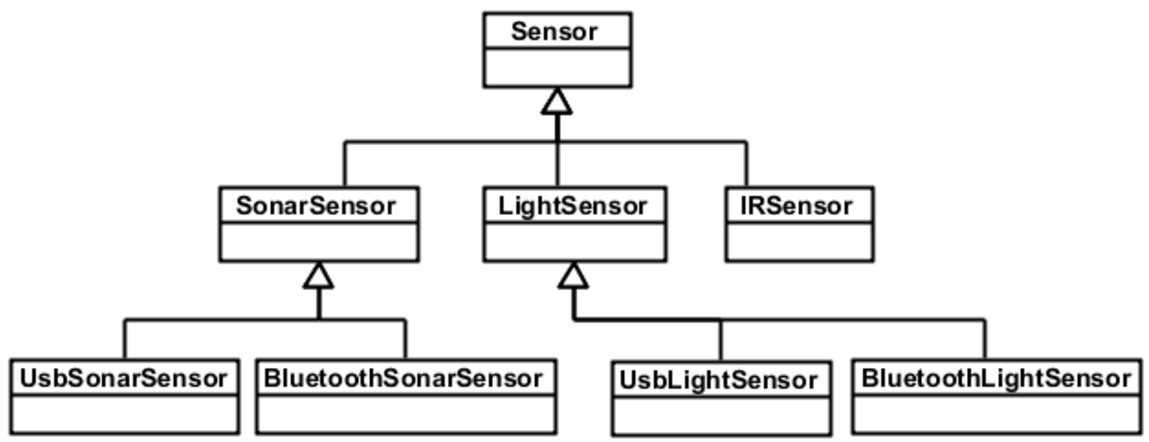
\includegraphics[width=0.8\textwidth]{noBridge.png}
\end{center}

Интерпретатор знает только про абстрактные базовые классы, модель робота во время выполнения подставляет конкретные реализации (что-то вроде паттерна <<Стратегия>> для каждого сенсора отдельно), все довольны. Однако с ростом поддерживаемых типов роботов и видов сенсоров становится печально --- количество конкретных классов по сути произведение количества сенсоров и типов связи. Тем более что формат передаваемых данных от типа сенсора более-менее не зависит\footnote{В реальной жизни это не совсем так, например, бывают синхронные и асинхронные сенсоры. Но всё равно форматов коммуникации меньше, чем видов сенсоров, так что для нашего примера сойдёт.}. Поэтому приходит в голову идея разделить концепции логической модели сенсора (например, <<инфракрасный датчик расстояния>>, возвращающий расстояния до препятствия в сантиметрах) и реализации запроса на устройство (например, у робота ТРИК запросить показания его датчика расстояния на таком-то порту). Получим вот такую архитектуру:

\begin{center}
    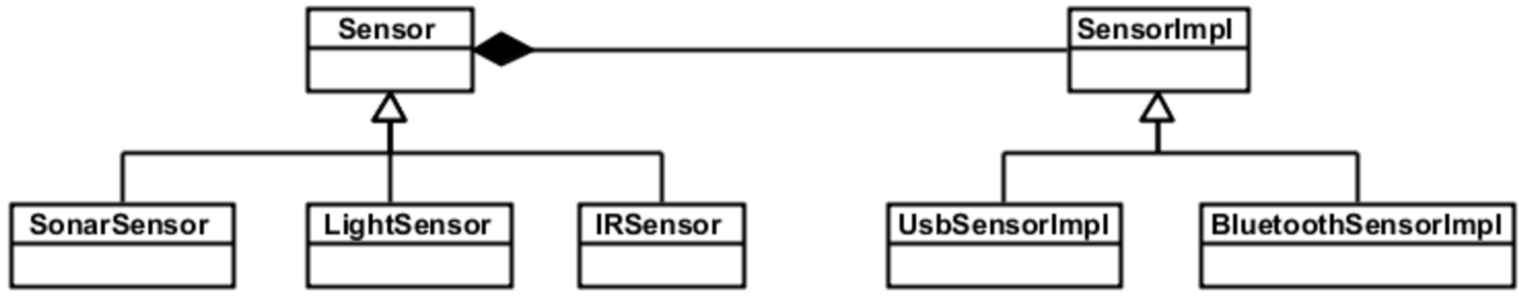
\includegraphics[width=0.8\textwidth]{bridge.png}
\end{center}

Слева иерархия логических сенсоров, которые ничего не знают об общении с роботом, но могут выполнять фильтрацию получаемых данных, нормализацию и т.д. Справа иерархия реализаций протоколов связи, которой по большей части всё равно, про какой сенсор идёт речь, но там происходит формирование и передача пакета с запросом на робот, получение и распаковка ответа. Между ними, собственно, <<мост>> --- отношение композиции (или агрегации), дающее каждому сенсору реализацию связи, через которую он может выполнять запросы на устройство.

Теперь у нас количество классов не произведение, а сумма количества видов сенсоров и способов связи. Для этого нам пришлось несколько пожертвовать гибкостью (теперь тут нет места, где можно было бы реализовать какой-то специфичный для сенсора и средства связи запрос) и немного усложнить архитектуру. Но часто оно того стоит.

\subsection{Мост (Bridge), общая структура}

Идея обобщается до вот такой схемы:

\begin{center}
    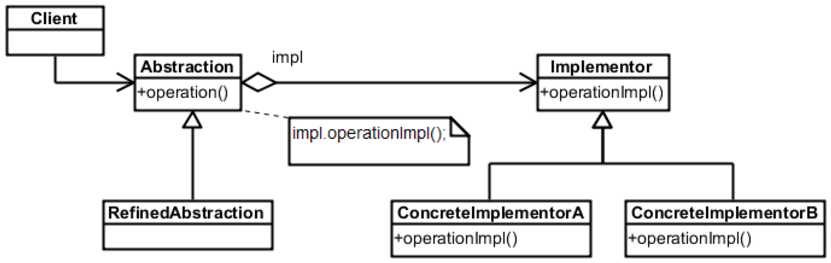
\includegraphics[width=0.8\textwidth]{bridgeGeneral.png}
\end{center}

Определение паттерна <<Мост>>, которое найдётся в интернете в большинстве случаев, звучит как <<Отделение абстракции от реализации>>. Сама эта фраза, к несчастью, ничего не значит (сразу возникает вопрос, не одно и то же ли <<Мост>> и принцип инкапсуляции из ООП), однако со структурной диаграммой начинает иметь смысл. Абстракция --- это то, с чем взаимодействует клиент, представляет высокоуровневые сущности. Реализация --- это то, что нужно абстракции для работы: как правило, низкоуровневые сущности, через которые абстракция реализует свою функциональность. Клиент про реализацию обычно ничего не знает, хотя может её создавать, чтобы сконфигурировать абстракцию. И абстракция, и реализация, как правило, представляют собой иерархии классов (в вырожденном случае одной абстракции и одноуровневой иерархии реализаций получаем паттерн <<Стратегия>>). Абстракция не знает (опять же, обычно) про конкретные реализации и всю работу выполняет через интерфейс Implementor, ссылка на который хранится в базовом классе.

Ещё один пример использования такой схемы --- библиотека пользовательских интерфейсов, где иерархией абстракций могла бы быть иерархия элементов управления (кнопки, текстовые поля и т.п.), а иерархией реализаций --- подсистема вывода графических примитивов (точек, линий и т.д.) под разные операционные системы.

Вообще же применяется этот паттерн в следующих ситуациях:

\begin{itemize}
    \item когда хочется разделить абстракцию и реализацию, например, для того, чтобы реализацию можно было легко менять во время компиляции или даже во время выполнения; при этом есть альтернативные способы это сделать:
    \begin{itemize}
        \item паттерн <<Стратегия>> --- когда у нас абстракция только одна, а реализации не образуют сложной иерархии;
        \item паттерн <<Заместитель>> --- когда нам не надо повысить уровень абстракции, а просто иметь возможность менять реализацию на лету (напомним, что в <<Proxy>> <<абстракция>> и <<реализация>> имеют одинаковый интерфейс);
    \end{itemize}
    \item поэтому говорят о паттерне <<Мост>> только тогда, когда и абстракция, и реализация могут расширяться новыми подклассами;
\end{itemize}

При этом одна реализация может быть разделяемой на несколько абстракций --- например, механизм copy-on-write для строк, реализованный в некоторых языках. Есть абстракция <<строка>>, которая сама никаких данных не содержит, и есть класс <<реализация строки>>. Если мы просто присвоили одну строку другой или скопировали строку, то абстракции просто указывают на одну реализацию. Но стоит одной из абстракций попытаться что-то в строке изменить, ей создаётся своя собственная реализация и изменения происходят уже в ней. Впрочем, в большинстве современных языков строки немутабельны.

\subsection{Детали реализации}

Наибольшую сложность при реализации этого паттерна представляет аккуратное разделение классов на абстракцию и реализацию, но это процесс творческий и сильно зависящий от задачи. Вам может повезти и разделение обнаружится естественным образом в предметной области (как в примере с оконными библиотеками выше), а может не повезти и паттерн <<Мост>> вообще окажется неприменим.

С технической точки зрения при реализации важно понять, как будет создаваться Implementor и как он будет внедряться в абстракцию. Тут возможны варианты:

\begin{itemize}
    \item абстракция сама понимает, какой конкретный Implementor ей нужен и создаёт его сама; быть может, с учётом параметров своего конструктора, конфигурации системы, или погоды за окном;
    \item вариант этого способа --- абстракция создаёт реализацию по умолчанию и предоставляет метод, позволяющий её подменить;
    \item более <<архитектурный>> вариант --- Implementor создаётся клиентом и передаётся в конструктор, или, лучше, создаётся IoC\footnote{Inversion of Control}-контейнером и подставляется в конструктор или свойство абстракции;
    \item ещё более <<архитектурный>> вариант --- в конструктор передаётся фабрика (про которую совсем скоро), с помощью которой абстракция создаёт Implementor по необходимости.
\end{itemize}

Использовать фабрику для создания Implementor-а в большинстве случаев может быть перебором, поскольку на ровном месте появляется ещё один промежуточный класс. Однако фабрика позволяет полностью отвязать и клиента, и абстракцию от реализации Implementor-а, вплоть до того, что Implementor может быть недоступен во время компиляции всей системы. Это позволяет, например, спрятать платформозависимые реализации Implementor-а --- в том же примере с оконной системой мы физически не можем компилироваться одновременно с реализацией под Windows и под Linux, поскольку ои наверняка завязаны на системные библиотеки.

\subsection{Pointer to Implementation (PImpl)}

Паттерн <<Pointer to Implementation (PImpl)>> --- пример языковой идиомы, или паттерна, специфичного для конкретного языка, в данном случае C++. Поэтому выделенного раздела он не заслуживает, и вообще не должен бы тут поминаться, но он близок по смыслу к паттерну <<Мост>>, и хоть один пример языкозависимого паттерна всё-таки, кажется, полезно разобрать. Pointer to Implementation можно рассматривать как вырожденный до минимума вариант паттерна <<Мост>> (или паттерна <<Стратегия>>, это больше вопрос точки зрения).

Итак, проблема C++ в том, что там нет нормальной модульной системы. Описания классов просто по соглашению между программистами делятся на два файла --- .hpp (или, по традиции, .h\footnote{От <<header>>, <<заголовочный файл>>.}), где класс просто декларируется (перечисляются его методы и поля), и .cpp, где класс реализуется (тут пишутся реализации методов). Когда кто-то хочет воспользоваться классом, он подключает просто текстуально .hpp-файл и получает себе предварительное объявление класса, которое потом линковщик использует, чтобы найти реализации методов, компилируемые отдельно\footnote{В отличие от большинства современных языков, компиляция C++ происходит пофайлово, то есть компилятор запускается как отдельный процесс на каждый .cpp-файл в системе, а потом линковщик, опять же запущенный как отдельный процесс, собирает всё, что получилось после компиляции, в один бинарник. Да, это действительно так медленно, как кажется из этого описания.}. Проблема в том, что в .hpp-файле методы класса могут не иметь реализации, но класс должен быть объявлен целиком, со всеми полями, private-методами, private-вложенными классами и т.п. Ну и получается, что если у класса один public-метод и двадцать полей, каждое своего типа, то клиент при подключении .hpp-файла должен (часто, хоть и не всегда) подключить ещё и двадцать .hpp-файлов с описанием типов полей, которые в свою очередь подключают по 20 заголовочных файлов и т.д. и т.п. Подключение, напомним, выполняется текстуально, так что компилятор при чтении невинного файла из 30 строк вынужден на самом деле разбирать полотно из 20000 строк, полученное <<склейкой>> в один файл всё дерево зависимостей. И это для каждого .cpp-файла, которых в нормальном проекте могут быть тысячи.

Для решения этой проблемы часто используются чисто языковые средства, типа предварительных объявлений, но они не позволяют решить архитектурную проблему --- клиентам всё же нужно зачем-то знать про детали реализации класса, который они используют. При изменении деталей реализации (как типов, так и просто имён полей или, например, параметров private-метода) клиент придётся перекомпилировать. И всех, кто от него зависит, и всех, кто зависит от тех, кто от него зависит. И так далее. Да, в C++ бывает так, что просто переименовываешь что-то в каком-нибудь классе-утилите, который используется много где в приложении --- и пару часов можно не работать, пока всё пересобирается.

Приходит на помощь паттерн <<Pointer to Implementation>>. Выносим всю private-часть нашего класса в отдельный класс, и объявляем его в .cpp-файле, где у нас была до этого реализация нашего класса, добавляем .hpp-файл предварительное объявление нашего нового класса, а в классе оставляем только одно поле, указатель на этот новый класс. Теперь все public-методы нашего класса используют этот самый указатель для получения объекта, который сделает за них всю содержательную работу:

\begin{center}
    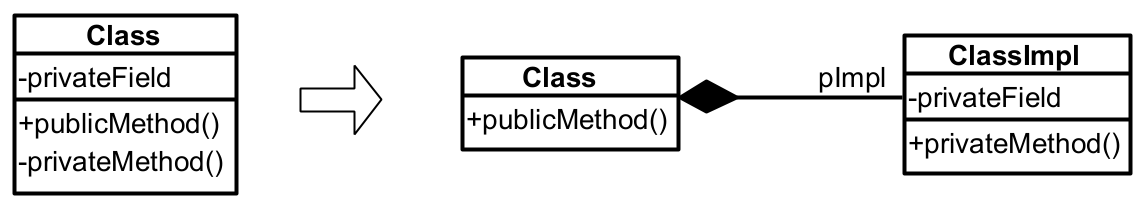
\includegraphics[width=0.7\textwidth]{pImpl.png}
\end{center}

Поскольку класс с реализацией объявлен в .cpp-файле, он компилируется только один раз и внешнему миру его не видно. Любое изменение там приведёт только к перекомпиляции его .cpp-файла, только одного. И зависимости этого класса подключаются в .cpp-файл, а не в .h-файл, так что клиентам не надо включать тысячи чужих зависимостей себе. Более того, мы можем смело добавлять новые поля --- поскольку класс-<<абстракция>> имеет только указатель на класс-<<реализацию>>, его размер от этого не изменится и мы не потеряем бинарную совместимость (то есть в памяти наш класс будет выглядеть всегда одинаково, и мы можем даже подсунуть новую реализацию в динамически загружаемой библиотеке, не пересобирая всё приложение). И главное, теперь мы можем менять реализацию как хотим, гарантированно не ломая ничего клиенту. 

Поэтому такой подход очень популярен в библиотеках на C++ --- например, библиотека Qt использует PImpl почти повсеместно. Это несколько усложняет отладку (чтобы посмотреть на внутреннее состояние объекта, надо пройти по ссылке на реализацию), добавляет оверхед на хранение указателя и вызовы методов, но обычно это того стоит (особенно в библиотеках, авторы библиотек могут спокойно рефакторить реализацию, не ломая бинарную совместимость).

\section{Паттерн <<Фабричный метод>>}

\subsection{Мотивирующий пример}

Перейдём к порождающим паттернам. Допустим, мы хотим сделать игру-стратегию наподобие Age of Empires или Warcraft. У нас есть юниты: мечник, всадник и лучник. У них разные характеристики и разное поведение, но есть и много общего, и мы, естественно, хотим работать с ними единообразно, для чего заводим им общий базовый класс <<Warrior>>:

\begin{center}
    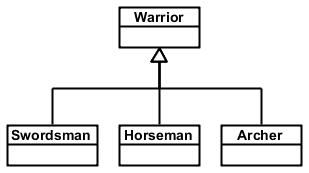
\includegraphics[width=0.4\textwidth]{warriors.png}
\end{center}

Теперь мы хотим реализовать класс <<Бараки>>, который будет производить юнитов, и, естественно, мы хотим написать содержательный код один раз, чтобы он работал со всеми типами юнитов. Однако проблема в том, что для вызова конструктора мы должны знать точный тип объекта --- виртуальных конструкторов не бывает, а в данном случае очень хочется. Не бывает не потому, что современные языки такие плохие, а потому, что в момент создания объекта определяется его тип времени выполнения, который как-то должен быть задан --- он и определяется конструктором, так что от вызова конструктора никуда не деться.

Однако если что-то очень хочется, народные умельцы найдут способ. Известен приём программирования, который называется <<Виртуальный конструктор>> (не делайте так, это плохая идея):

\begin{minted}{c++}
enum WarriorId { SwordsmanId, ArcherId, HorsemanId };

class Warrior
{
public:  
    Warrior(WarriorId id)
    {
        if (id == SwordsmanId) p = new Swordsman;
        else if (id == ArcherId) p = new Archer;
        else if (id == HorsemanId) p = new Horseman;
        else assert(false);
    }
    virtual void info() { p->info(); }
    virtual ~Warrior() { delete p;  p = 0; }
private:
    Warrior* p;
};
\end{minted}

В базовом классе Warrior заводится поле, которое будет указывать на реальный объект, и конструктор, который инициализирует это поле в зависимости от каких-то факторов (в нашем случае идентификатор требуемого типа юнита). Все запросы к объекту базового класса просто перенаправляются объекту <<настоящего>> класса (как info() в нашем примере). То есть Warrior, помимо того, что является базовым классом для конкретных юнитов, играет роль прокси, который позволяет выбрать реализацию, и даже при желании менять её во время выполнения. На диаграмме классов это выглядит как-то так:

\begin{center}
    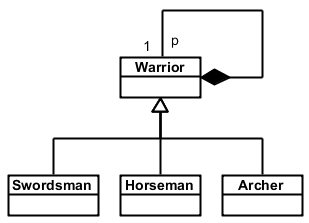
\includegraphics[width=0.35\textwidth]{warriorVirtualCtor.png}
\end{center}

Плохо это тем, что нарушается принцип единственности ответственности (Warrior слишком умный), добавляется ненужный уровень косвенности (и затраты на вызовы методов через прокси), и для каждого юнита хранится два комплекта полей Warrior, один из которых не используется (один в прокси, другой в проксируемом объекте, который наследуется от Warrior), да ещё и Warrior больше нельзя сделать абстрактным.

Можно улучшить эту идею, заменив извращённый конструктор на статический метод (делайте так иногда, это адекватный, хотя и не всегда лучший способ решения проблемы):

\begin{center}
    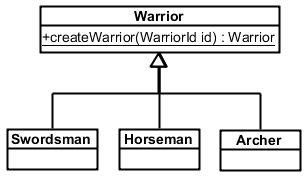
\includegraphics[width=0.35\textwidth]{warriorFactoryMethod.png}
\end{center}

Метод createWarrior всё так же содержит выбор конструктора и всё так же хочет знать, кого ему создавать, поэтому принимает id. Но по крайней мере Warrior можно оставить абстрактным и нет никаких проблем с вызовами через прокси (правда, мы теперь во время выполнения не можем поменять тип юнита, но это обычно и не надо, а если будет надо, можно сделать более явным образом).

\subsection{Фабричный метод (Factory Method), общая структура}

Следующий шаг развития идей модельного примера приведёт нас уже к настоящему фабричному методу: сделать метод создания не статическим, а виртуальным, и заменить цепочку if-ов на вызов виртуального метода. На диаграмме классов это выглядит так:

\begin{center}
    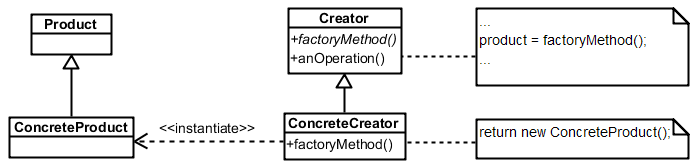
\includegraphics[width=0.9\textwidth]{factoryMethod.png}
\end{center}

Creator --- это класс, которому надо создать объект, но он заранее не знает, какого тот типа. Тогда Creator может объявить себе абстрактный метод factoryMethod (тот самый фабричный метод, в честь которого назван паттерн), и дальше пользователи Creator-а могут унаследоваться от него, переопределив этот factoryMethod так, чтобы он возвращал нужный объект. Обычно его реализация пишется в одну строчку и сводится к вызову конструктора. Product --- это общий интерфейс всех возможных продуктов, он является типом возвращаемого значения factoryMethod. ConcreteProduct-ов может быть сколько угодно, для каждого из них надо будет объявить ConcreteCreator, чтобы тот его создавал и тем самым параметризовал Creator подклассом Product-а.

Кажется, что это может понадобиться очень редко, но на самом деле паттерн применяется весьма  часто, в ситуациях, когда Creator делает много содержательной работы, но часть её делегирует Product-у, и Product может делать эту работу по-разному (например, <<Фабричный метод>> может создавать стратегию для паттерна <<Стратегия>>, где Creator будет играть роль Context-а). Это на самом деле очень удобный способ параметризовать один объект другим объектом, не передавая его явно извне (например потому, что объект должен создавать Product-ы в больших количествах и по ходу работы).

В примере со стратегией Product-ом был бы Warrior, ConcreteProduct-ами были бы Archer, Swordsman и Horseman, а Creator-ом --- бараки, которые могли бы быть уточнены подклассами <<Бараки мечников>>, <<Поле для лучников>> и <<Конюшни>>. Каждый подкласс реализовывался бы в одну строку, что несколько неуклюже, но решает нашу проблему с переиспользованием кода бараков для разных типов юнитов. Вот ещё пример, из книги Банды Четырёх:

\begin{center}
    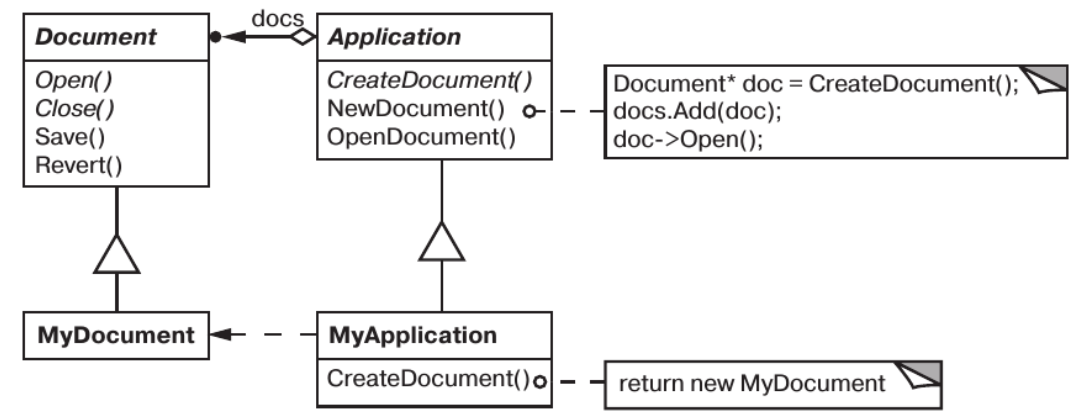
\includegraphics[width=0.85\textwidth]{factoryMethodForTextEditor.png}
\end{center}

Тут речь идёт о фреймворке, который позволяет создавать редакторы разных форматов файлов (например, текстовых и изображений). Есть абстрактный базовый класс Document, от которого мы должны отнаследоваться, чтобы реализовать свой формат, и абстрактный класс Application, в котором делается много содержательной работы (типа открытия и создания документа). От него мы должны унаследоваться и переопределить фабричный метод CreateDocument(), чтобы он возвращал наш вид документов, всё остальное фреймворк сделает сам. 

\subsection{Детали реализации}

 Creator на самом деле вовсе не обязан быть абстрактным --- он вполне может предоставлять реализацию фабричного метода по умолчанию. Это может быть полезно, если фабричный метод является на самом деле точкой расширения на будущее --- пользователи Creator могут переопределить создаваемый объект, но не обязаны это делать. Это же и минус такого подхода --- пользователи могут забыть переопределить фабричный метод и получить внезапное поведение по умолчанию, а не ошибку компиляции.

 Фабричный метод вполне может принимать параметры и даже выбирать в зависимости от них тип создаваемого объекта. 
 
 Если язык поддерживает инстанцирование по прототипу (например, JavaScript или Smalltalk), можно ничего и не выбирать, и даже не наследовать конкретный Creator --- просто параметризуем Creator прототипом и делаем его клон при необходимости.

 Маленькая тонкость, про которую, тем не менее, надо помнить --- Creator не может вызывать фабричный метод в конструкторе, так что если хочется параметризовать действия, совершаемые в конструкторе, придётся использовать что-то ещё. Почему --- в момент вызова конструктора предка (Creator) конструктор потомка (ConcreteCreator) ещё не отработал и потомок находится в неконсистентном состоянии. Вызов любого виртуального метода в конструкторе предка, не только фабричного метода, приведёт либо к ошибке компиляции, либо, что гораздо хуже, к внезапным и трудноотлаживаемым ошибкам времени выполнения.

 Один из способов решения этой проблемы --- если язык позволяет, заменить наследование параметризацией шаблона (как мы уже делали в паттерне <<Стратегия>>). В Java это работать не будет, создать объект типа-параметра шаблона там нельзя. В C\# и C++ это вполне валидная альтернатива классической реализации.

 Ну и конечно, вместо фабричного метода можно использовать лямбда-функцию, которая будет по требованию создавать Product-ы, и передавать её Creator-у при инициализации. В современных языках это, пожалуй, лучший на самом деле способ реализации этого паттерна, который в Книжке не описан --- в те времена, когда она писалась (и даже когда выходили её переиздания), лямбда-функций в нормальных языках ещё не было.

\section{Паттерн <<Абстрактная фабрика>>}

\subsection{Мотивирующий пример}

Вернёмся к текстовому редактору, на примере которого рассказывалось большинство паттернов. Теперь наша задача --- поддержать разные стили оформления пользовательского интерфейса. Нам хочется иметь возможность выбирать стиль при запуске редактора. Например, если запустили под Windows, используется внешний вид элементов, типичный для Windows, если под Linux, то внешний вид, типичный для местного оконного менеджера (В Java AWT, кстати, была такая функциональность). И хочется иметь возможность удобно расширять набор стилей (хотя бы потому, что оконных менеджеров под Linux очень много). Поэтому мы начнём с того, что реализуем абстрактные элементы и конкретные реализации под каждый из пока поддерживаемых стилей:

\begin{center}
    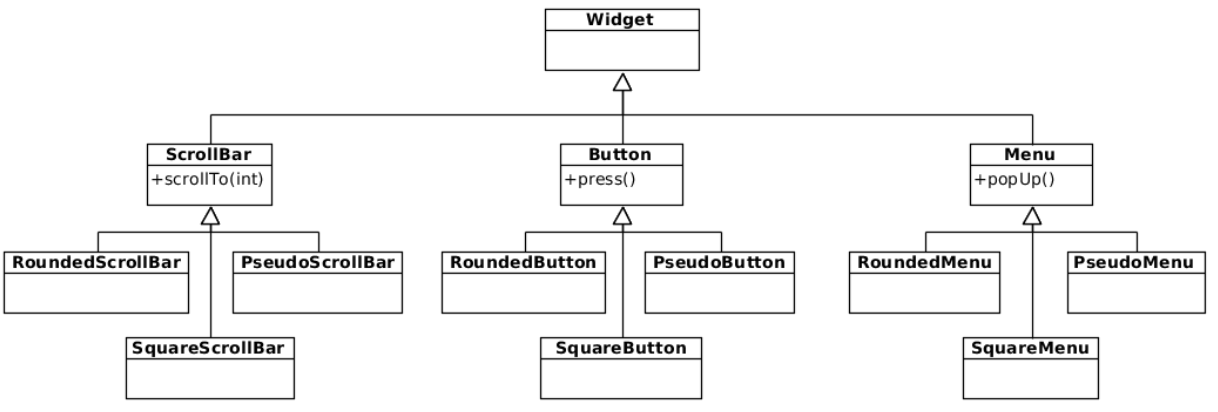
\includegraphics[width=0.9\textwidth]{widgets.png}
\end{center}

Очень напоминает ситуацию в паттерне <<Мост>> до рефакторинга, и кажется, что можно избежать квадратичного числа классов, но тут ничего не выйдет --- разные элементы управления должны реально выглядеть по-разному, и там должен быть какой-то произвольный код, который никуда из них не вынести. Поэтому будем жить с этим.

Проблема возникает в том, как эту иерархию использовать в коде редактора. Наивный подход --- при создании каждого окна смотреть, какой стиль используется, и в зависимости от этого создавать те или иные конкретные элементы управления, --- упирается в то, что окон в редакторе может быть очень много, и если в каждом написать гигантский switch, нам быстро надоест. И добавление нового стиля превратится в пытку, с тысячей ошибок времени выполнения, когда мы где-то забыли добавить вариант.

Поэтому предлагается вынести код создания объектов в отдельный класс, и использовать его везде, где надо создавать объект. Например, если нам надо создать полосу прокрутки, мы пишем не \mintinline{c++}|ScrollBar* bar = new RoundedScrollBar;|, а \mintinline{c++}|ScrollBar* bar = guiFactory->createScrollBar();|. Гигантский switch можно в таком случае реализовать в guiFactory, и передавать её везде, где надо создавать элементы --- это позволит при добавлении нового стиля поменять только одно место в коде, и избежать копипаста. А можно вспомнить, что если у вас где-то есть гигантский switch, то вы можете переделать его в вызов виртуальной функции, и получить уже настоящий паттерн <<Абстрактная фабрика>>:

\begin{center}
    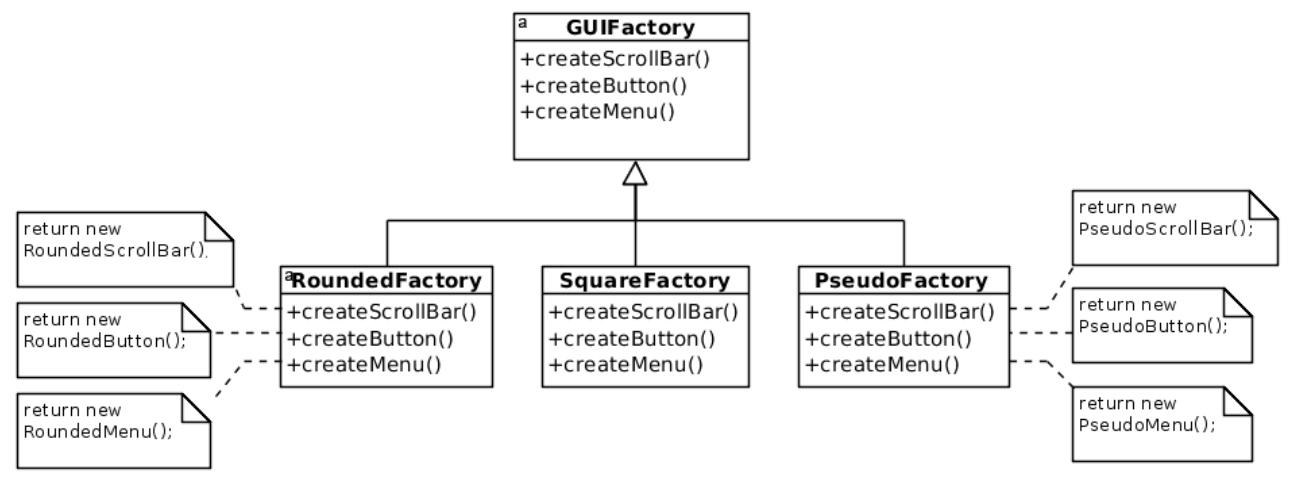
\includegraphics[width=0.95\textwidth]{widgetFactory.png}
\end{center}

Один гигантский switch нам всё-таки будет нужен --- при старте приложения мы смотрим, какой визуальный стиль нам нужен, и выбираем, какую фабрику создать. Дальше отдаём эту фабрику всем, кто планирует создавать элементы управления, они запрашивают у неё элемент, она возвращает нужный. Каждая фабрика --- это набор однострочных методов, которые просто вызывают конструктор нужного типа.

\subsection{Абстрактная фабрика (Abstract Factory), общая структура}

Эта идея обобщается до следующей схемы:

\begin{center}
    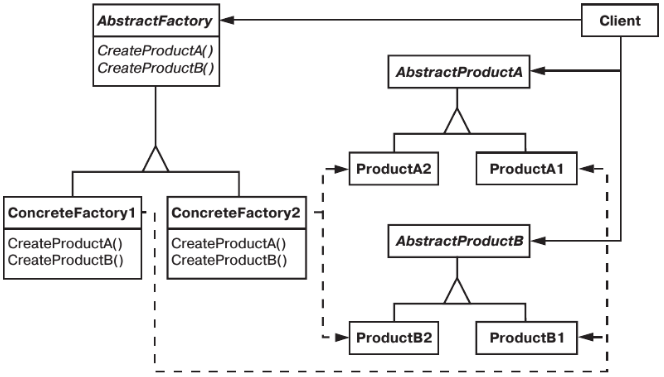
\includegraphics[width=0.7\textwidth]{abstractFactory.png}
\end{center}

Есть набор продуктов (в нашем примере --- разных элементов управления), продукты образуют иерархии, но разные типы продуктов могут быть никак не связаны друг с другом. Есть абстрактная фабрика, декларирующая умение создавать абстрактные продукты, и наследующиеся от неё конкретные фабрики, каждая из которых умеет создавать свой вид конкретного продукта каждого типа. Клиент, желающий создавать продукты, знает только про абстрактные продукты и про абстрактную фабрику. Кто-то ещё должен уметь создать конкретную фабрику --- либо сам клиент, либо кто-то ещё, и отдать её клиенту.

Это позволяет очень хорошо изолировать конкретные классы от тех мест, где они будут использоваться --- клиент знает только про абстракции (которые, скорее всего, просто интерфейсы), а конкретные продукты ему могут быть не видны вообще, и даже не быть доступны во время компиляции клиента (например, подключаться в виде плагина). Чтобы подменить вид продуктов, достаточно просто передать клиенту новую фабрику. Единственное, что клиент уже мог успеть насоздавать продуктов, поэтому если хочется изменить вид продуктов уже после инициализации клиента, надо делать механизм, позволяющий его переинициализировать (что как правило хлопотно, поэтому многие приложения просят себя перезапустить после столь радикальных изменений).

При этом, правда, добавление нового типа продуктов (то есть AbstractProductC) довольно хлопотно, придётся в каждую существующую фабрику добавить новый метод, и поправить код клиента, чтобы он им пользовался. Добавление нового вида продукта (то есть ProductA3,  ProductB3 и т.д.) требует добавления новой фабрики, что обычно гораздо проще. Кстати, наличие общего интерфейса у каждого типа продукта гарантирует их совместимость, то есть при добавлении нового продукта он гарантированно будет вести себя как все остальные --- это бесплатный бонус при использовании паттерна <<Абстрактная фабрика>>.

Применяется абстрактная фабрика в следующих ситуациях (достаточно истинности одного условия, чтобы задуматься о применении паттерна):

\begin{itemize}
    \item система не должна зависеть от того, как создаются входящие в неё объекты: если мы хотим создать один объект, то это не страшно, а вот если продукт требует инициализации здоровенной подсистемы, логику инициализации может иметь смысл вынести в фабрику просто для того, чтобы спрятать её от клиента;
    \item система должна конфигурироваться типом объектов, с которыми она будет работать --- это всяческая поддержка стилей, вариантов реализации (например, в примере с роботами из паттерна <<Мост>> фабрика могла создавать объекты для управления конкретным типом робота), поддержка плагинов;
    \item взаимосвязанные объекты должны использоваться вместе --- фабрика не даст перепутать и создать все кнопки в стиле Windows, кроме одной;
    \item хотите предоставить библиотеку объектов, раскрывая только их интерфейсы, но не реализацию --- тогда создать объекты с помощью конструкторов у клиента физически не выйдет, фабрика будет играть роль этакой библиотеки конструкторов, через которую клиент и будет получать объекты.
\end{itemize}

Фабрику можно рассматривать как класс, состоящий из нескольких реализаций паттерна <<Фабричный метод>>. Принципиальное отличие в том, что в паттерне <<Фабричный метод>> предполагается, что класс, где этот самый фабричный метод находится, сам делает массу содержательной работы и использует фабричный метод только для дополнительного конфигурирования. <<Абстрактная фабрика>> же --- это выделенный класс, цель существования которого --- только создание объектов и ничего больше.

\subsection{Детали реализации}

Абстрактная фабрика хорошо комбинируется с паттерном <<Одиночка>>, который мы рассмотрим следующим. Скорее всего, фабрика одна на всю систему, и вместо того, чтобы старательно передавать её всюду, где она нужна, можно сделать её доступной глобально. Однако в обсуждении паттерна <<Одиночка>> мы рассмотрим, почему это может быть плохой идеей, так что пользоваться таким приёмом надо с большой осторожностью.

Если типов продуктов много, то можно рассмотреть возможность не создавать кучу подклассов абстрактной фабрики, а сделать <<универсальную>> фабрику, которая во время выполнения параметризуется создаваемыми продуктами. Для этого можно использовать паттерн <<Прототип>> (про который чуть позже), тем более если в языке реализации так принято (например, JavaScript). А можно параметризовать фабрику лямбда-функциями, которые будут создавать объект. А можно, если язык позволяет, сделать фабрику шаблоном и конкретные типы передавать при инстанцировании шаблона как параметры-типы (но это куда как страшнее, чем использование аналогичного приёма в паттерне <<Стратегия>>, потому что типов продуктов обычно много и параметров шаблона будет тоже много --- поэтому не разу не встречал такого способа на практике). А ещё можно использовать рефлексию и параметризовать фабрику объектами-типами (например, Class в Java или Type в .NET), из которых с помощью рефлексии создавать продукты, но не нужно --- использовать рефлексию без нужды всегда плохая идея.

Ещё методы создания объектов в фабрике могут принимать параметры, исходя из которых выбирать, объект какого типа они хотят создать. Однако, в отличие от аналогичного приёма в паттерне <<Фабричный метод>>, это может сильно запутать дело. Есть соблазн с помощью параметра выбирать одно из семейств (например, вместо CreateScrollBar и CreateButton сделать метод CreateWidget, принимающий, что за элемент управления надо создать), но это очень рискованная идея, потому что нарушается типобезопасность --- клиент без идей, продукт какого типа ему вернули, и компилятор не может проверить, что правильного.

\section{Паттерн <<Одиночка>>}

\subsection{Мотивирующий пример}

Мотивирующий пример паттерна <<Одиночка>> --- предыдущий паттерн. У нас есть фабрика элементов управления, и мы знаем, что будем использовать одну эту фабрику во всём приложении, причём в тысяче разных мест. Мы могли бы передавать её как параметр везде, но нам бы быстро надоело (тем более что есть фабрика элементов управления, которую надо передавать везде, конфиг, который надо передавать везде, подсистема логирования, которую надо передавать везде, и т.д.). Сделать её глобальной переменной не вариант, потому что глобальные переменные это плохо, тем более что никто не гарантирует, что кто-нибудь возьмёт и создаст свою другую фабрику, и всё испортится.

\subsection{Одиночка (Singleton), общая структура}

На помощь приходит паттерн <<Одиночка>>, задачи которого --- как раз обеспечить глобальный доступ к некоторому ресурсу и гарантировать, что этот ресурс присутствует в системе в одном экземпляре. Структура у него очень проста:

\begin{center}
    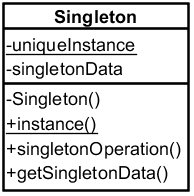
\includegraphics[width=0.2\textwidth]{singleton.png}
\end{center}

Уникальность экземпляра гарантируется тем, что у класса private-конструктор, и public-статический метод instance(), который возвращает (и при необходимости инициализирует) статическую переменную uniqueInstance. Поскольку конструктор недоступен извне, создать экземпляр может только метод instance(). В остальном это обычный класс, то есть у него могут быть поля, методы и т.п.

В принципе, структура может быть более сложной --- instance может принимать параметры, а сам Singleton иметь потомков. Тогда instance в зависимости от переданных параметров может создавать одного из потомков, тем самым обеспечивая конфигурируемость системы.

\subsection{Детали реализации}

Самое интересное в паттерне <<Одиночка>> --- это реализация. Как правило, желательно обеспечить ленивость инициализации экземпляра --- если объект большой и потенциально может никому не понадобиться, нет смысла его заранее создавать. А это приводит к некоторым интересным проблемам с многопоточностью, потому что если одиночку пытаются инициализировать два потока сразу, нельзя, чтобы получилось два экземпляра. Обычно в этом курсе мы избегаем таких технических подробностей, оставляя это на обсуждение на курсах по многопоточному программированию, но конкретно про многопоточную реализацию <<Одиночки>> очень любят спрашивать на собеседованиях, поэтому всё-таки обсудим.

Итак, простая реализация Одиночки могла бы выглядеть вот так:

\begin{minted}{java}
public class Singleton {
    private static Singleton instance;

    private Singleton () {}

    public static Singleton getInstance() {
        if (instance == null) {
            instance = new Singleton();
        }
        return instance;
    }
}
\end{minted}

Тут статический метод getInstance() при первом вызове создаёт экземпляр класса, сохраняет его в instance и возвращает, а при последующих вызовах возвращает уже его. Если два потока одновременно пытаются обратиться к неинициализированному одиночке, они могут оба проверить instance на null, оба войти в тело if-а и оба создать instance, при этом удастся записать в instance значение только кому-то одному. При этом менее удачливый поток может успеть вернуть <<плохой>> instance, что нарушит инвариант одиночки и потенциально всё испортит.

Это легко исправить, сделав инициализацию статического поля в момент загрузки класса, а не первого обращения:

\begin{minted}{java}
public class Singleton {
    private static Singleton instance = new Singleton();

    private Singleton () {}

    public static Singleton getInstance() {
        return instance;
    }
}
\end{minted}

Среда времени выполнения всех нормальных языков гарантирует инициализацию статических полей без каких-либо гонок, но вот порядок инициализации статических полей не определён, и мы потеряли ленивость --- экземпляр одиночки будет создан тут же.

Это можно поправить и с сохранением ленивости:

\begin{minted}{java}
public class Singleton {
    private static Singleton instance;

    public static synchronized Singleton getInstance() {
        if (instance == null) {
            instance = new Singleton();
        }
        return instance;
    }
}
\end{minted}

В других языках программирования тоже есть что-то, аналогичное synchronized в Java --- это просто монитор на весь метод (например, в C\# того же эффекта можно добиться, заключив всё тело метода в lock). Теперь все обращения к getInstance() синхронизируются, и только один поток может в данный момент времени пытаться создать одиночку. Проблема решена, но решена не оптимальным образом: гонка в принципе может возникнуть только при инициализации одиночки, тогда как этот способ требует синхронизации при каждом обращении к getInstance(), даже когда всё давно инициализировалось и никакой гонки быть не может.

Правильное решение выглядит несколько сложнее и называется Double-checked locking\footnote{Хорошая статья про то, насколько аккуратно всё надо делать и почему: \url{https://www.cs.umd.edu/~pugh/java/memoryModel/DoubleCheckedLocking.html} (дата обращения: 23.08.2021г).}:

\begin{minted}{java}
public class Singleton {
    private static volatile Singleton instance;

    public static Singleton getInstance() {
        Singleton localInstance = instance;
        if (localInstance == null) {
            synchronized (Singleton.class) {
                localInstance = instance;
                if (localInstance == null) {
                    instance = localInstance = new Singleton();
                }
            }
        }
        return localInstance;
    }
}
\end{minted}

Если одиночка ещё не проинициализирован, берём замок, и дальше внутри замка повторяем проверку --- потому что пока мы его берём, другой поток мог успеть быстрее. Ещё важно не забыть volatile на instance --- это заставит компилятор сгенерировать команды синхронизации при чтении и записи в instance, чтобы избежать проблем с перестановкой инструкций на процессоре. Что добавляет заметный оверхед на чтение в строке, где мы читаем instance в localInstance (впрочем, существенно меньший, чем synchronized), и именно желание этот оверхед минимизировать заставило нас тут этот самый localInstance и завести --- без него из instance пришлось бы читать дважды.

Как видим, внезапно хорошая реализация синглтона требует нетривиальных познаний в архитектуре процессора (а процессоры бывают разные, так что надо ещё понимать, подо что вы программируете), так что встаёт вопрос, стоит ли оно того. Возможно, обойтись статическим инициализатором будет проще.

Есть ещё одна модификация паттерна <<Одиночка>>, которая называется <<Multiton>> (уж не знаю, как это перевести на русский). Это реестр одиночек --- возвращает по заданному ключу уникальный объект, создавая объекты при необходимости и гарантируя их уникальность. Структурно он выглядит примерно так:

\begin{center}
    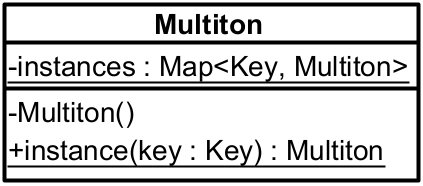
\includegraphics[width=0.3\textwidth]{multiton.png}
\end{center}

Всё остальное там устроено так же, как в одиночке (со всеми проблемами многопоточности, помноженными ещё на необходимость синхронизации доступа в Map), и полезно это особенно тогда, когда у Multiton есть наследники. Впрочем, ни разу не встречал такой конструкции на практике.

\subsection{Критика}

Поскольку <<Singleton>>, по крайней мере, по опыту автора, больше походит на антипаттерн, перечислим его проблемы аж в отдельном разделе.

\begin{itemize}
    \item По сути, <<Одиночка>> --- хитрая глобальная переменная. Если он мутабельный, то в любом месте программы в него можно что-то записать, а потом в любом месте программы считать, что сильно запутывает поток данных. С немутабельными одиночками дела обстоят получше, но всё же, порядок инициализации может быть нетривиальным, в коде этого не видно, так что система может сломаться, если вы поменяли пару строк местами, и это будет очень сложно отладить.
    \item <<Одиночка>> усложняет тестирование, поскольку его невозможно подменить тестовой заглушкой (Mock-объектом) и ему самому невозможно внедрить зависимости. Если одиночка зависит от других классов системы, то при запуске тестов они честно проинициализируются, что как минимум нарушит изоляцию тестируемой части системы, как максимум сделает написание юнит-тестов вообще невозможным (представьте себе кнопку запуска ядерной ракеты, реализованную как одиночка). И это большая проблема, потому что если на какой-то кусок кода нет тестов, можно смело считать, что он не работает.
    \item <<Одиночка>> нарушает принцип единственности ответственности. Он одновременно отвечает за свой жизненный цикл и делает полезную работу, причём, как мы видели, поддержание правильного жизненного цикла может требовать относительно много нетривиального кода, который и сам по себе сложно поддерживать.
    \item То, что изначально планируется как <<Одиночка>>, имеет тенденцию внезапно появляться в системе в нескольких экземплярах, и тогда рефакторинг по переделке <<Одиночки>> в честную передачу нужного объекта во все места, которые его используют, может занять много времени и сил. Например, однажды мы разрабатывали систему визуального моделирования, где был репозиторий, хранящий все созданные в системе диаграммы и элементы --- его, казалось бы, естественно было сделать одиночкой, тем более что он был нужен практически всем. Первые пару лет всё даже шло хорошо, но внезапно возникло требование сравнивать разные версии диаграмм, а это было проще всего реализовать, создав рядом второй репозиторий. Пришлось убирать паттерн <<Одиночка>> и много чего болезненно рефакторить.
\end{itemize}

На самом деле, часть проблем с паттерном может решить IoC-контейнер. Большинство IoC-библиотек умеют управлять жизненным циклом лежащих в контейнере объектов сами, и делать это правильно, с учётом многопоточности и ленивости создания. То есть вы просто описываете обычный класс и регистрируете его в контейнере как одиночку, а он уже создаёт объект, поддерживает его уникальность и т.д. Правда, не гарантируется, что никто больше не создаст такой объект, но если все получают объекты только из контейнера, то всё хорошо. Зато если он перестанет быть одиночкой, достаточно будет просто сказать контейнеру об этом.

\subsection{Паттерн <<Ленивая инициализация>> (Lazy Initialization)}

Ещё один близкий паттерн, не заслуживающий своего раздела --- <<Ленивая инициализация>>. Это штука, сильно напоминающая <<Одиночку>>, но не имеющая целью сделать создаваемый объект уникальным или глобально доступным. <<Ленивая инициализация>> отвечает только за создание объекта по требованию. Структурно она устроена почти как <<Одиночка>> --- есть <<обёртка>>, которая умеет создать настоящий объект при необходимости (например, принимает в конструктор лямбда-функцию создания), и имеет что-то вроде метода instance(), которая создаёт объект и запоминает его, чтобы возвращать в дальнейшем. Нужно это для рационального использования ресурсов, прежде всего --- если ресурсоёмкое действие может не выполниться вовсе, не стоит его выполнять раньше времени. Однако кое-какие вещи без ленивости не сделать в принципе --- например, бесконечные структуры данных. Также на курсах по функциональному программированию любят показывать примеры программ, которые при ленивых вычислениях быстро дают ответ, а при неленивых вообще зацикливаются.

В отличие от паттерна <<Одиночка>>, ленивая инициализация используется практически повсеместно. Например, в Haskell (следуя нормальной стратегии $\beta$-редукции в $\lambda$-исчислении) ленивость лежит в основе модели вычислений, там все выражения считаются только в тот момент, когда это абсолютно необходимо. В других языках обычно ленивые вычисления требуют явного указания, например, в .NET для этого есть библиотечный тип \mintinline{csharp}{Lazy<T>}, а в F\# даже синтаксический сахар для него --- ключевое слово lazy. Нередки и ленивые структуры данных --- бесконечную последовательность простых чисел, например, можно сделать хоть на старой Java, с помощью итераторов, в более современных языках для этого встречается более развитая поддержка. На самом деле, даже Just-In-Time-компиляция, которую использует большинство современных языков --- это тоже подвид ленивых вычислений.

С точки зрения реализации Lazy имеет те же проблемы, что и Singleton с многопоточностью. Точно так же, требуется обеспечить отсутствие гонок при вызове инициализатора и отсутствие лишних синхронизаций, когда объект уже проинициализирован. Double-checked locking может быть применён и здесь (опять-таки, при должном уровне внимательности и понимания архитектуры целевой машины, то есть осторожно).

\section{Паттерн <<Пул объектов>>}

\subsection{Мотивирующий пример}

Ещё один паттерн не из книги Банды Четырёх, но близкий по духу <<Одиночке>> и <<Приспособленцу>> --- <<Пул объектов>>. В качестве мотивирующего примера возьмём одно из его применений в реальной жизни --- механизм работы с потоками в .NET (практически точно такой же есть и в Java, и в других языках).

В стандартной библиотеке .NET потоки отображаются напрямую в потоки операционной системы, поток для программиста представляет класс Thread. У Thread есть конструктор, который принимает функцию (лямбду или ссылку на метод), создаёт поток и запускает переданную ему функцию там. Когда функция заканчивает работу, поток уничтожается. 

Для всех популярных операционных систем создание нового потока --- это дорогая операция. Требуется выделение памяти под стек потока (а это несколько мегабайт оперативной памяти, так что создать тысячу потоков может быть плохой идеей только из-за этого), памяти в пространстве ядра под управляющие структуры, требуется вызов планировщика (и дополнительные затраты на планирование потока), и главное, всё равно на процессоре обычно не очень много ядер, а иметь больше потоков, чем ядер, нет особого смысла --- им всё равно не дадут поработать\footnote{Тут есть небольшая тонкость --- сейчас принято относиться к потоку как к программной абстракции ядра процессора, но в былые времена (то есть в конце 90-х и начале 2000-х, когда проектировались модели многопоточности в современных языках и закладывались традиции) поток был абстракцией задачи, которая могла делаться параллельно с другими задачами (и, например, заблокироваться, ожидая события). Поэтому современные стандартные библиотеки иногда пытаются натянуть новое миропонимание на старый код, из-за чего местами выглядят неконсистентно. Например, в современном .NET настоятельно не рекомендуется использовать класс Thread, хоть в библиотеке он есть.}.

Решение --- пул потоков. В .NET это класс ThreadPool, <<одиночка>>, который создаёт заранее N потоков, которые работают в бесконечном цикле <<взять задачу из очереди --- сделать задачу --- если задач в очереди нет, подождать, пока появятся, иначе перейти в начало цикла>>. У ThreadPool есть метод QueueUserWorkItem, который принимает задачу на исполнение, например, \mintinline{csharp}|ThreadPool.QueueUserWorkItem(() => Console.WriteLine("Goodbye, world!"))|. Если есть свободный поток. переданная задача тут же запускается в нём, если нет, ждёт своей очереди. Вызвавшему возвращается объект класса Task, который он может использовать, чтобы дождаться результата и получить результат. Если очередь слишком большая и все потоки заняты, создаются новые потоки, а если очередь пуста и потоков больше N, лишние заканчивают работу. N обычно выбирается согласно числу ядер на той машине, на которой запущена программа.

\subsection{Пул объектов (Object pool), общая структура}

Обобщается это всё в паттерн, структурно похожий на <<Приспособленца>>, но без попыток манипуляции состоянием и разделения элементов пула. Есть класс, отвечающий за поддержание объектов из пула (ThreadPool в нашем примере), он создаёт объекты при необходимости (Thread в нашем примере), удаляет их и возвращает по требованию клиентов (либо, как ThreadPool, не возвращает, а сам использует их, чтобы делать полезную работу). Применяется он в ситуации, когда объекты создавать сложно, но каждый объект нужен лишь ненадолго и может быть переиспользован.

При этом желательно, чтобы на поддержание объектов в пуле не требовалось много ресурсов, либо объектов в пуле было мало. Например, в ThreadPool обычно единицы либо десятки потоков, а если бы их было, скажем, десять тысяч, паттерн был бы неприменим. Или пул из сетевых соединений, где мы на всякий случай создаём их сразу 50000 --- это плохая идея.

\subsection{Детали реализации}

Обычно наличие в языке сборки мусора упрощает реализацию --- как, например, в паттерне <<Компоновщик>>, где мы долго рассуждали про проблемы с удалением разделяемых поддеревьев. В <<Пуле потоков>> наоборот --- сам пул держит ссылки на хранящиеся в нём объекты, поэтому для управления их временем жизни может потребоваться дополнительный подсчёт числа использующих их клиентов или ещё какой-то механизм, позволяющий понять, когда объект можно удалить. Также стоит помнить, что если язык использует сборку мусора, в нём, скорее всего, минимальные накладные расходы на выделение памяти --- например, в .NET это просто одна арифметическая операция, увеличение указателя на начало невыделенной области кучи. Так что если вы хотите сделать пул объектов, чтобы сэкономить время на выделение памяти, может получиться даже хуже, чем было.

Как и в <<Одиночке>>, в случае с пулом объектов тоже надо помнить о многопоточности. Сам пул обычно (но не всегда) <<Одиночка>>, и обращения к методам пула могут происходить из разных потоков, что, в силу необходимости манипуляции пулом объектов, может приводить к гонкам. Обычно методы пула сами требуют синхронизации.

\section{Паттерн <<Прототип>>}

\subsection{Мотивирующий пример}

Положим, мы теперь разрабатываем редактор нотной записи. Там есть нотный стан, на который надо уметь из палитры вытаскивать ноты разных длительностей. Хочется иметь возможность легко расширять палитру и не писать произвольный код создания каждого вида нот в гигантском switch при начале операции drag-and-drop. Можно снабдить палитру кучей фабрик, но есть более элегантное решение, которое, к тому же, позволит нам легко копировать уже существующие части нотной записи. Мы сделаем всем объектам, которые могут быть на нотном стане, метод Clone(), и в палитру добавим прототипы этих объектов --- то есть по одному объекту каждого типа, которые можно будет клонировать и тащить на нотный стан:

\begin{center}
    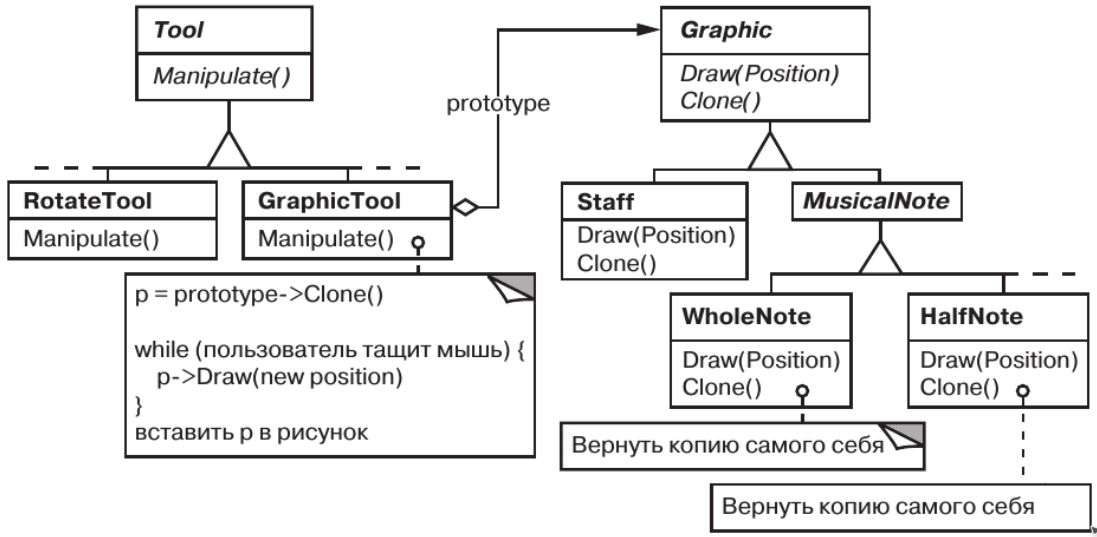
\includegraphics[width=0.9\textwidth]{musicalEditor.png}
\end{center}

Класс Graphic --- общий базовый класс (или интерфейс) для всего, что есть в палитре и на нотном стане, он декларирует возможность рисовать элемент и клонировать элемент, порождая его точную копию. GraphicTool --- это клиент Graphic, он реализует операции над элементами, в частности, drag-and-drop. При клике мышью на палитре он вызывает Clone() элемента палитры, на который кликнули, тот создаёт ему копию себя, которую и тащат на нотный стан.

\subsection{Прототип (Prototype), общая структура}

Обобщается идея до паттерна <<Прототип>> с вот такой, по сути очень простой, структурой:

\begin{center}
    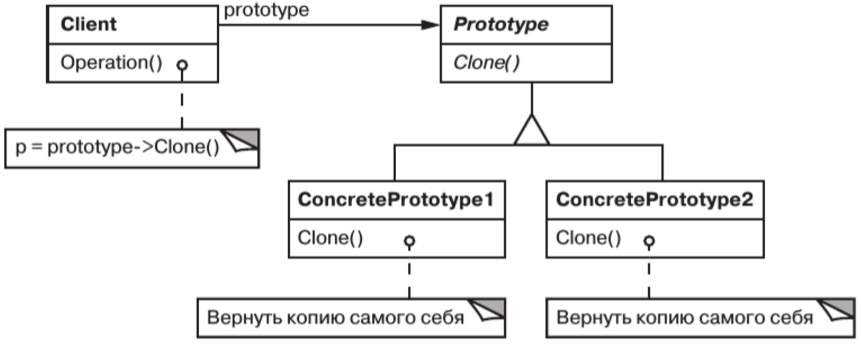
\includegraphics[width=0.8\textwidth]{prototype.png}
\end{center}

Фактически весь паттерн сводится к тому, что декларируется метод Clone() и предлагается использовать его для порождения копий нужных объектов. Обратите внимание, что это тоже помогает устроить что-то вроде виртуального конструктора: Clone() виртуальный, и создаёт копию объекта того класса, от которого он в итоге вызвался --- клиент про тип объекта ничего не знает.

\subsection{Детали реализации}

Прототип можно реализовать через рефлексию, если она поддерживается в языке. Вытащить тип времени выполнения и запустить его конструктор рефлексией вполне можно, и даже скопировать значения полей. Но, как обычно, рефлексией стоит пользоваться только если очень надо, тут может быть проще и лучше самим Clone() реализовать.

Прототип обычно полезен не сам по себе, а с каким-то способом быстро получить нужный прототип. В примере про музыкальный редактор это делала палитра, определяя по координатам клика мышью, какой элемент надо создать. Иногда применяют реестр прототипов --- ассоциативное хранилище (быть может, <<Одиночка>>), где можно легко найти и клонировать нужный объект.

Самое хитрое в паттерне --- это реализация Clone(). Во-первых, надо ответить себе на вопрос, хотим ли мы глубокое или мелкое копирование:

\begin{itemize}
    \item глубокое копирование копирует объект, объекты, на которые он ссылается, объекты, на которые ссылаются они, и т.д., то есть весь граф по ссылкам;
    \item мелкое копирование копирует только сам объект, оставляя ссылки такими, какие они были.
\end{itemize}

Глубокое копирование --- это то, что ожидается любыми нормальными людьми, поэтому если нет веских причин поступить иначе, надо, чтобы Clone() выполнял именно его. Однако реализовать глубокое копирование, особенно если в графе копируемого объекта есть круговые ссылки, может быть довольно нетривиально --- надо делать честный обход, запоминать ссылки на уже скопированные объекты и т.д. И работать это, естественно, будет гораздо дольше, чем мелкое копирование, особенно если граф объектов большой. И мелкое копирование вполне можно использовать, если вся структура немутабельна и от разделения объектов никому плохо не будет.

Немного хакерский способ быстро реализовать глубокое копирование --- взять объект, сериализовать его с помощью какой-нибудь библиотеки сериализации (в память, естественно, не на диск), а потом десериализовать. Тут, правда, надо следить за идентичностью результата --- например, если в объекте был какой-то id-шник, то библиотека сериализации скопирует его как он есть, и мы получим два разных объекта с одним id-шником, что наверняка закончится трагедией. Однако никто не мешает все поля, которые у оригинала и у клона должны быть разными, подправить после клонирования руками. Почему способ хакерский --- потому что это быстро и просто реализовать, но работать будет заведомо медленнее, чем реализация Clone() вручную. Так что в продакшн-коде так лучше не делать.

Ещё один тонкий момент --- это если в клоне должны быть ещё какие-то, кроме идентификатора, значения, отличные от оригинала. Возникает соблазн сделать методу Clone() параметры, которыми можно было бы проинициализировать созданный клон, однако если посмотреть на стандартные библиотеки, где этот паттерн реализован, никто так не делает. Clone() не принимает параметры неспроста --- каждому конкретному прототипу для инициализации, скорее всего, потребуется свой набор параметров (не сейчас, так в будущем). Ну а объявить Clone() в базовом классе, просто объединив множества всех нужных параметров --- очень неООПшно и хрупко (придётся менять интерфейс каждый раз, когда у кого-то из подклассов меняется какой-то параметр).

\end{document}